\appendix[nosub] % use \appendix if there are subappendices

%appendix text
%-------------------------------------------------------------------------------------------
\chapter{รูปอุปกรณ์เครื่องมือวัดและทดสอบ}
\begin{center}
 \begin{figure}[H]
		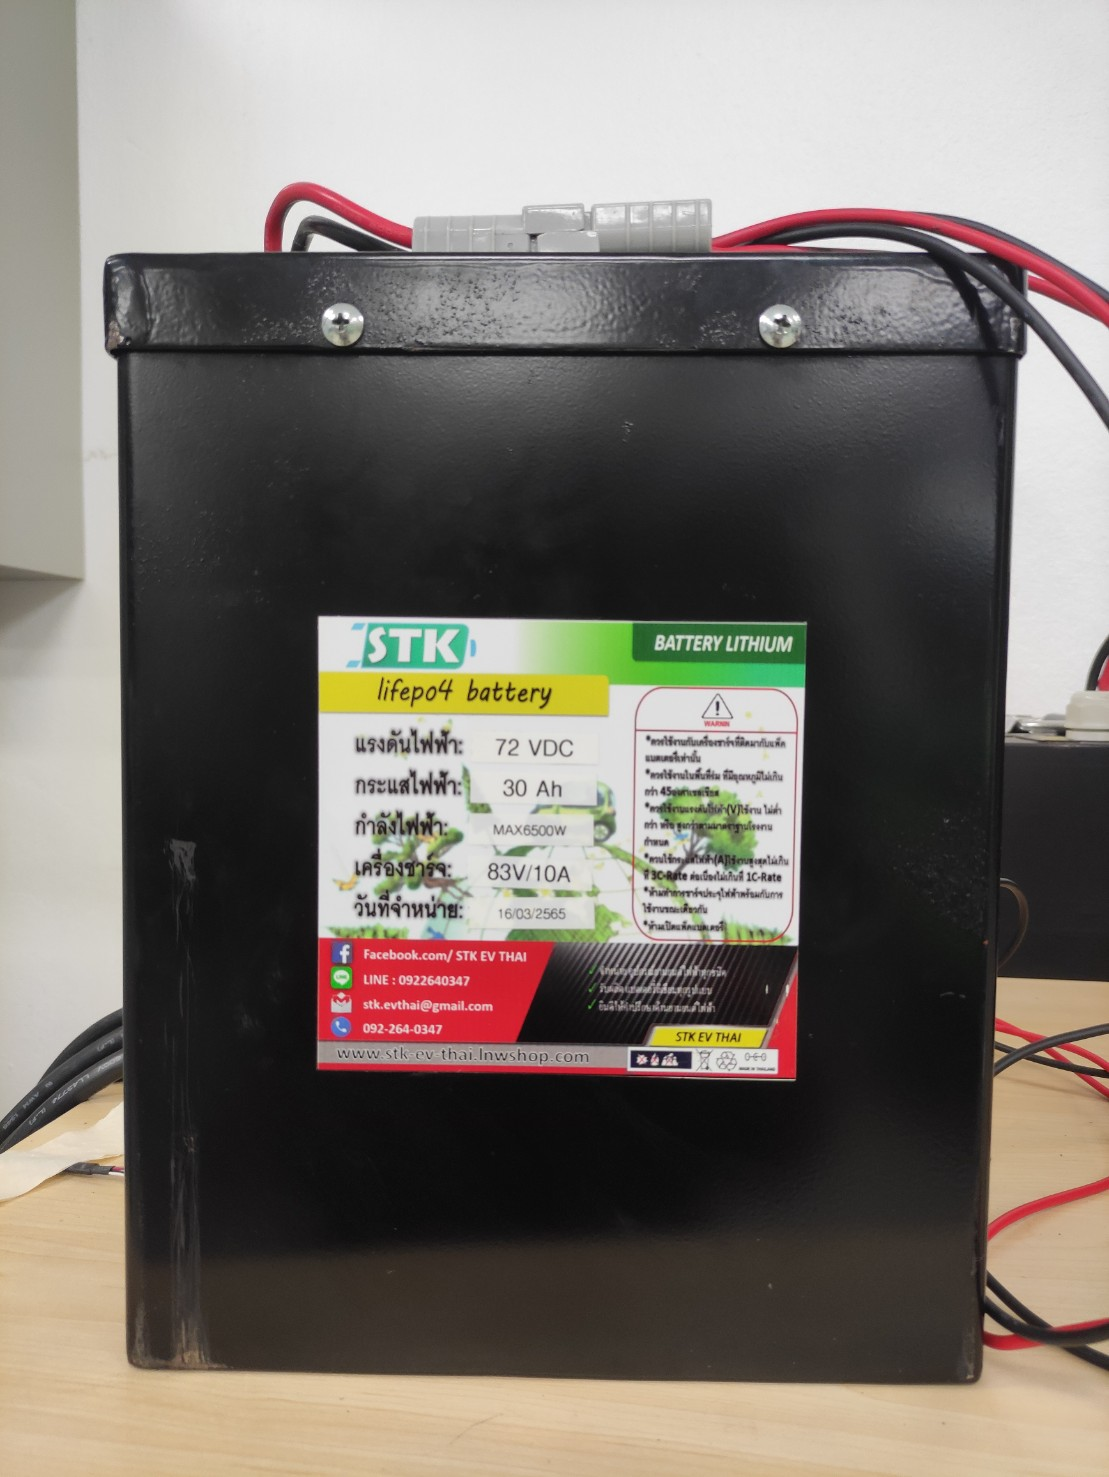
\includegraphics[width=0.5\linewidth]{Chapters/img/Battery_72V30Ah.jpg}
		\centering
		\captionsetup{justification=centering,margin=2cm}
		\caption{แบตเตอรี่สำหรับจักยานยนต์ไฟฟ้า 72V30Ah}
	\end{figure}
	\begin{figure}[H]
		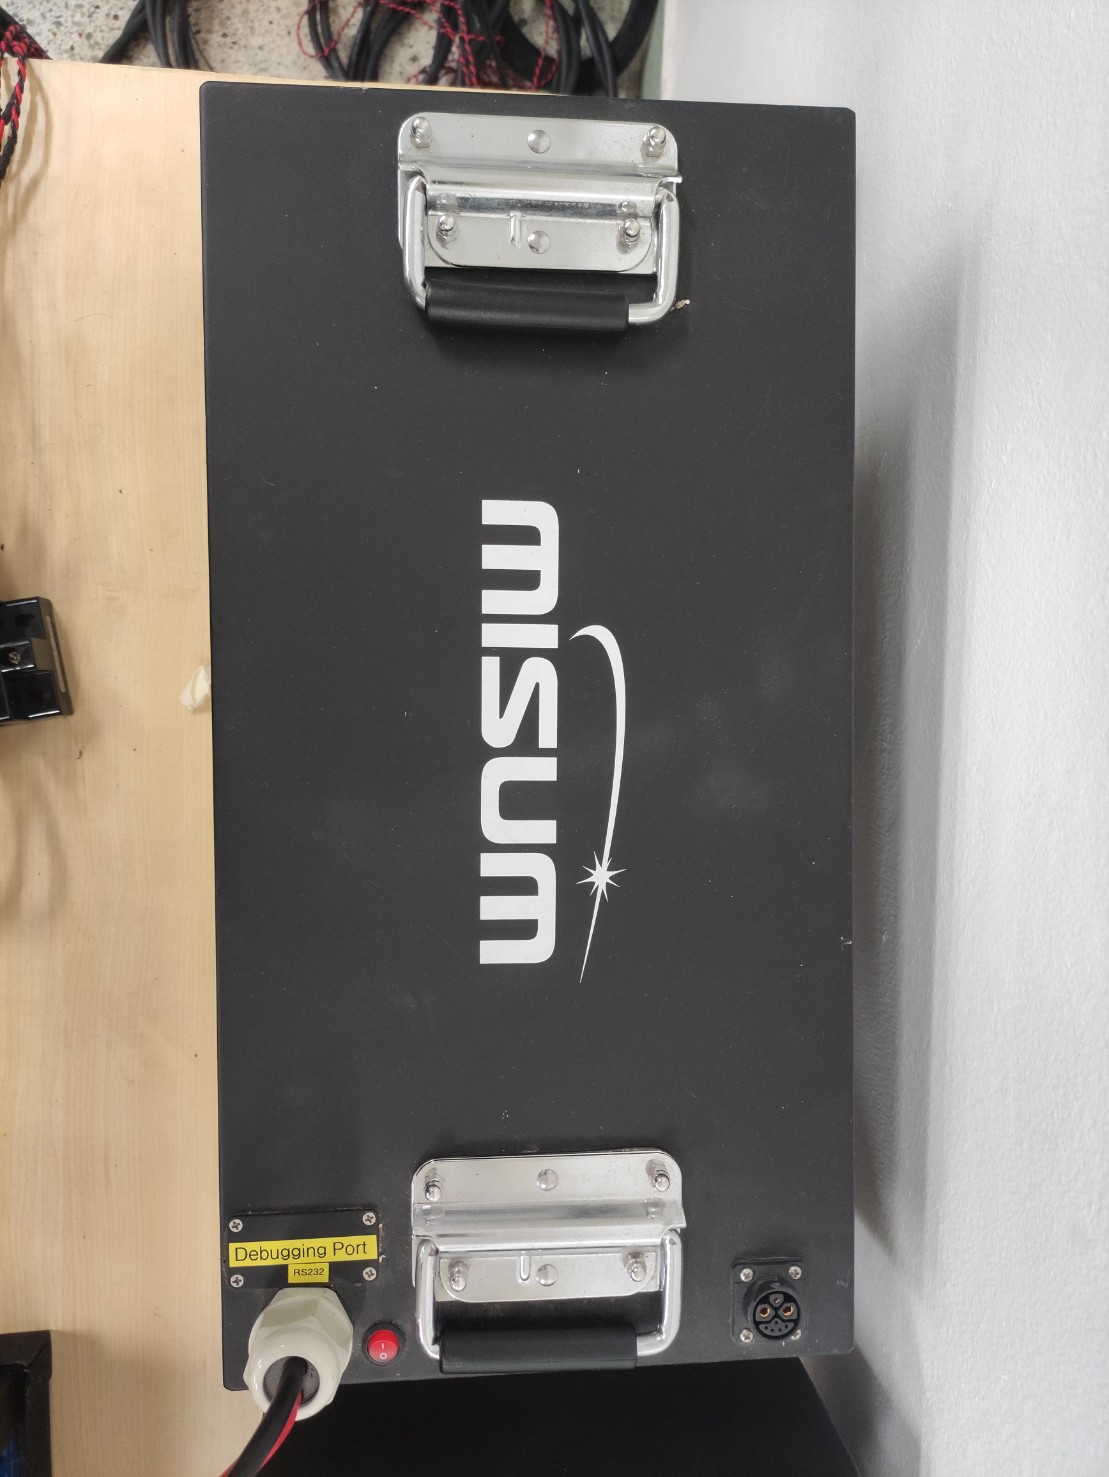
\includegraphics[width=0.5\linewidth]{Chapters/img/Battery_72V60Ah.jpg}
		\centering
		\captionsetup{justification=centering,margin=2cm}
		\caption{แบตเตอรี่สำหรับสามล้อไฟฟ้า 72V60Ah}
	\end{figure}
	\begin{figure}[H]
		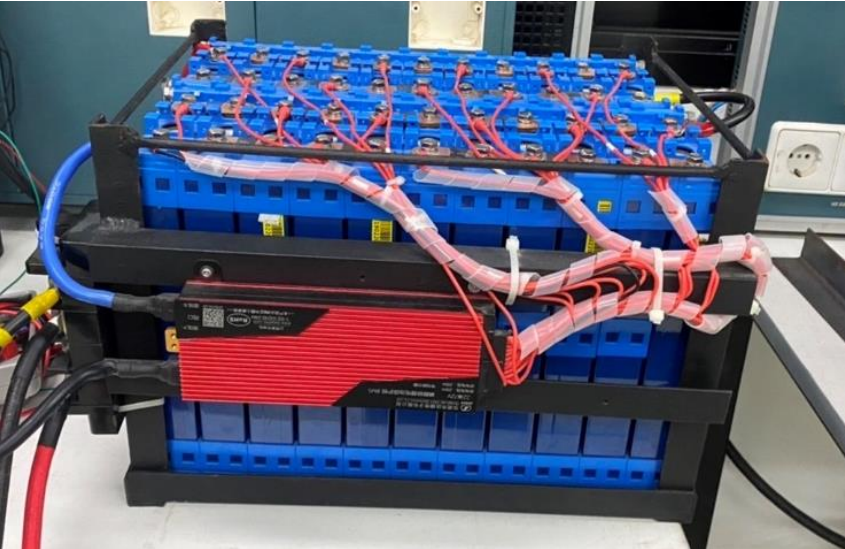
\includegraphics[width=0.5\linewidth]{Chapters/img/Battery_72V72Ah.jpg}
		\centering
		\captionsetup{justification=centering,margin=2cm}
		\caption{แบตเตอรี่ 72V72Ah}
	\end{figure}
	\begin{figure}[H]
		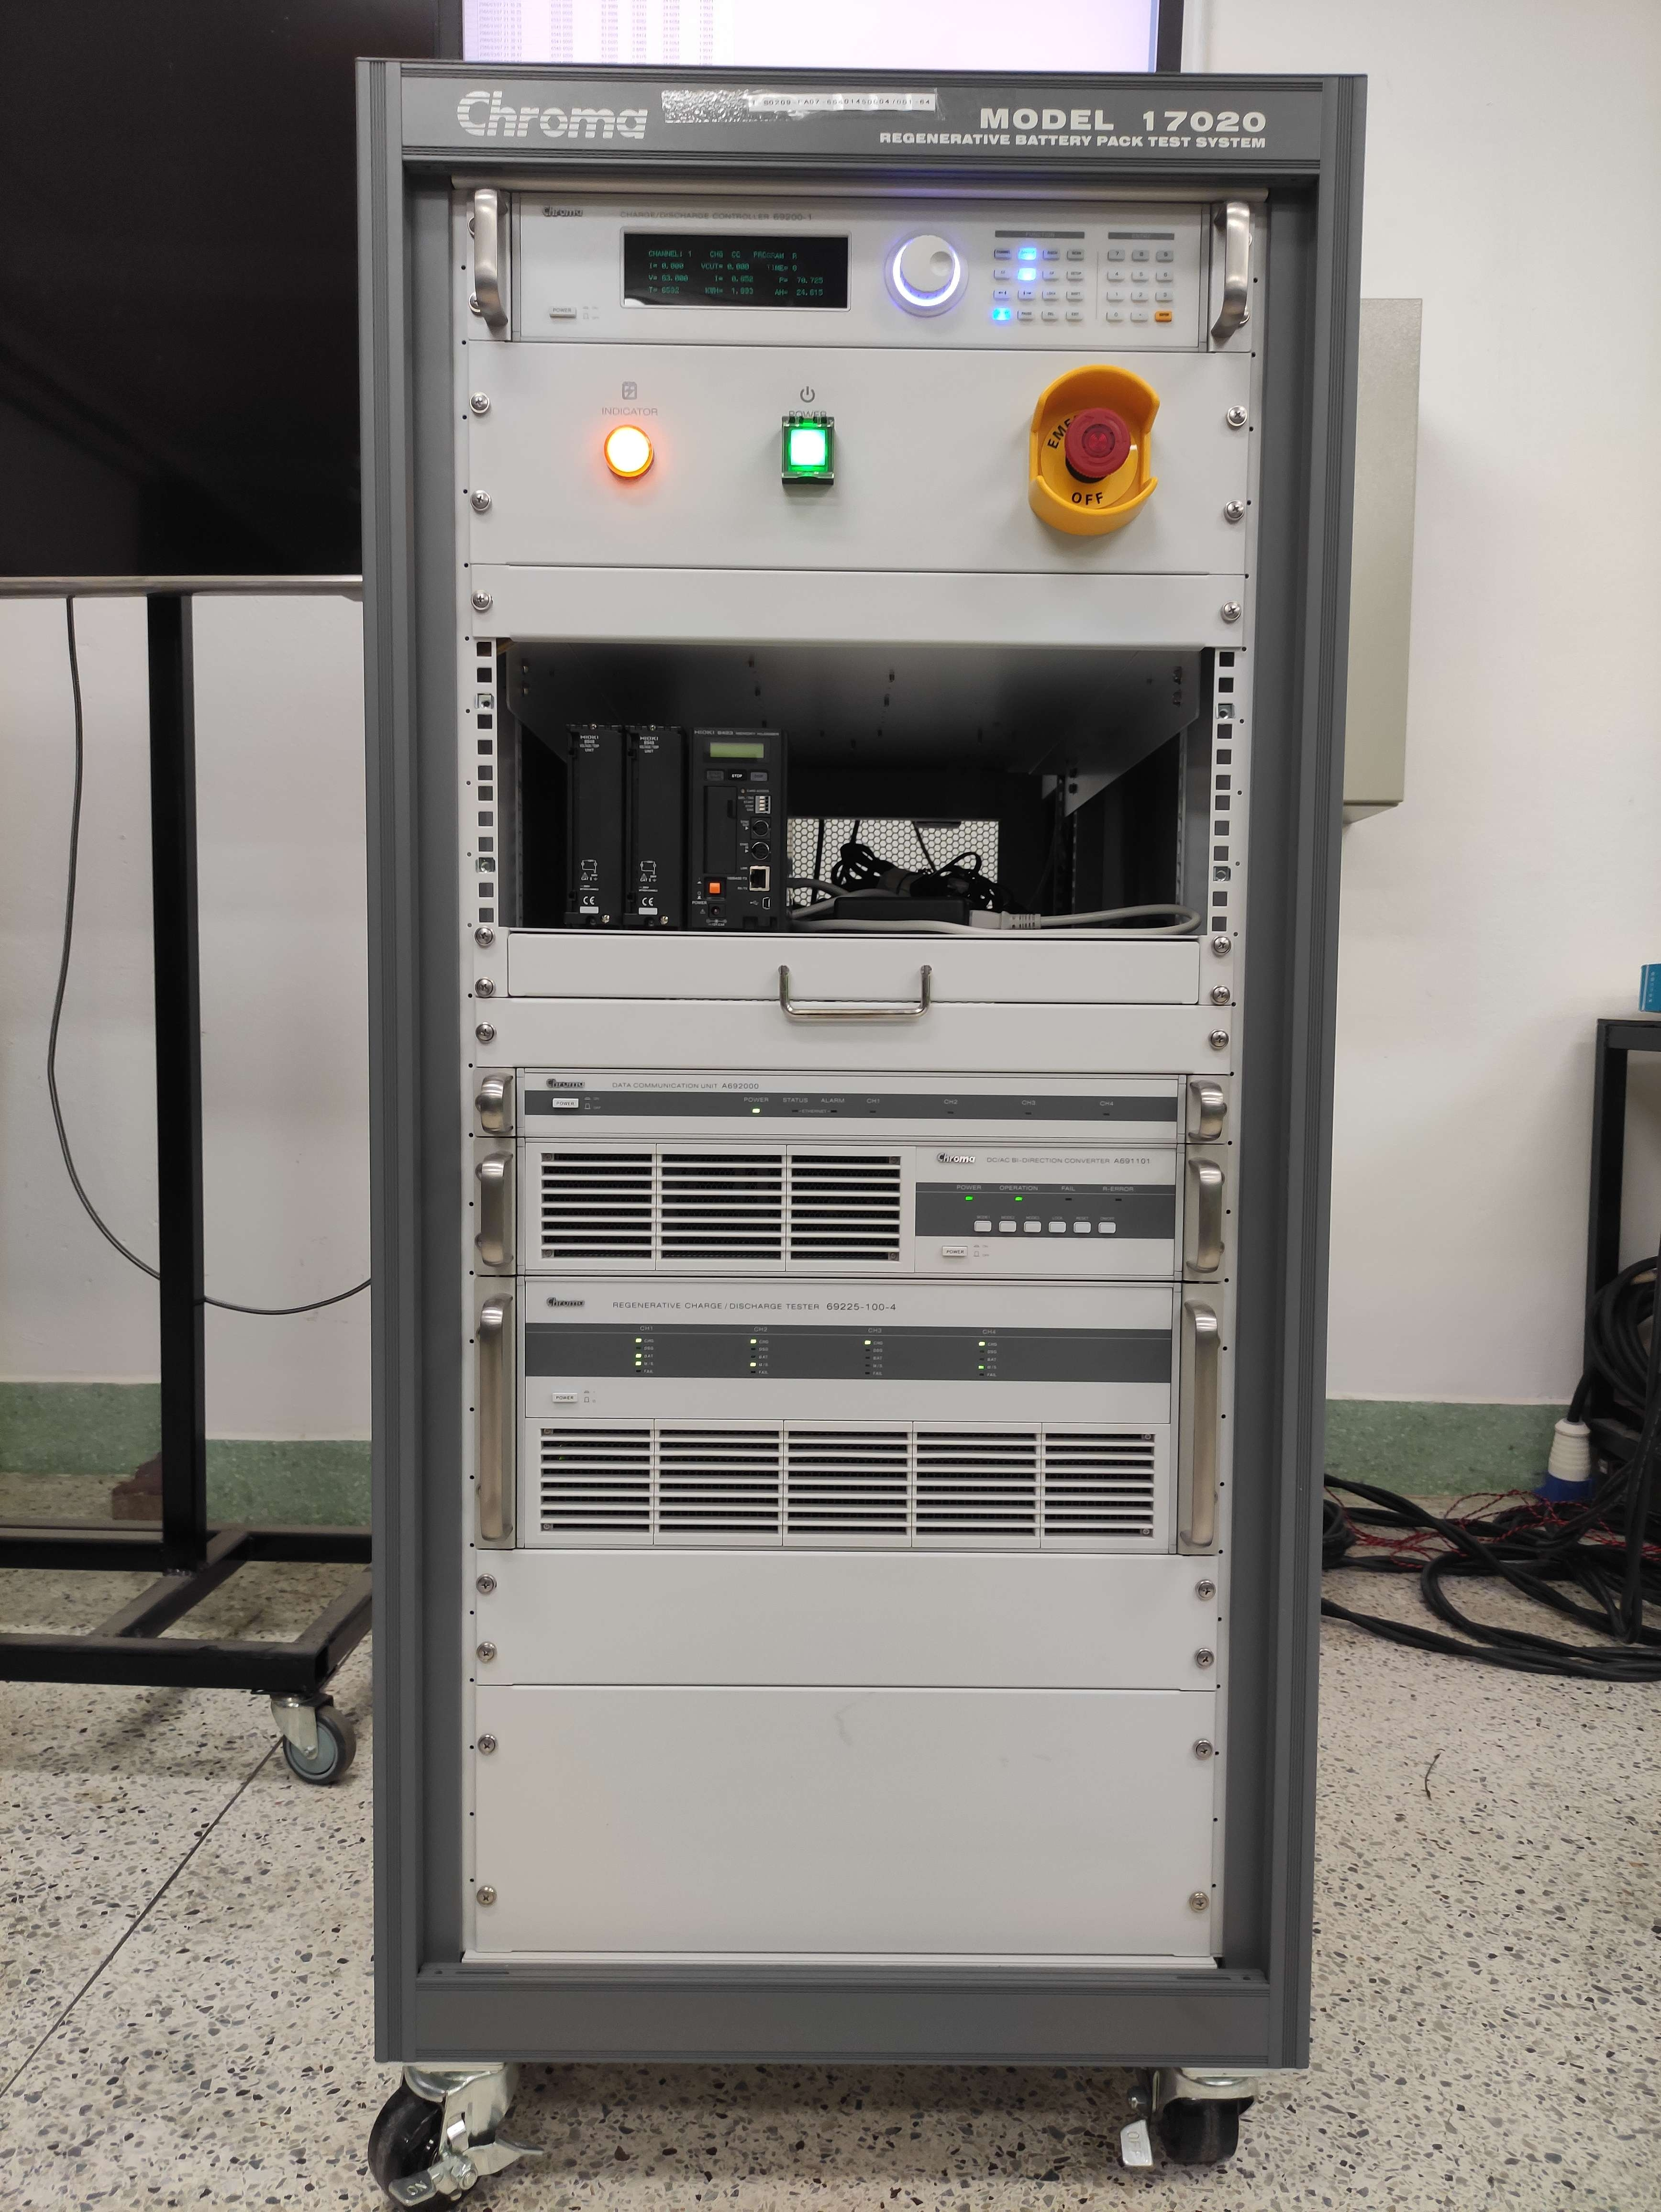
\includegraphics[width=0.5\linewidth]{Chapters/img/Chroma_17020.jpg}
		\centering
		\captionsetup{justification=centering,margin=2cm}
		\caption{เครื่องทดสอบแบตเตอรี่ Chroma model 17020}
		\label{fig:Chroma model 17020}
	\end{figure}
	\begin{figure}[H]
		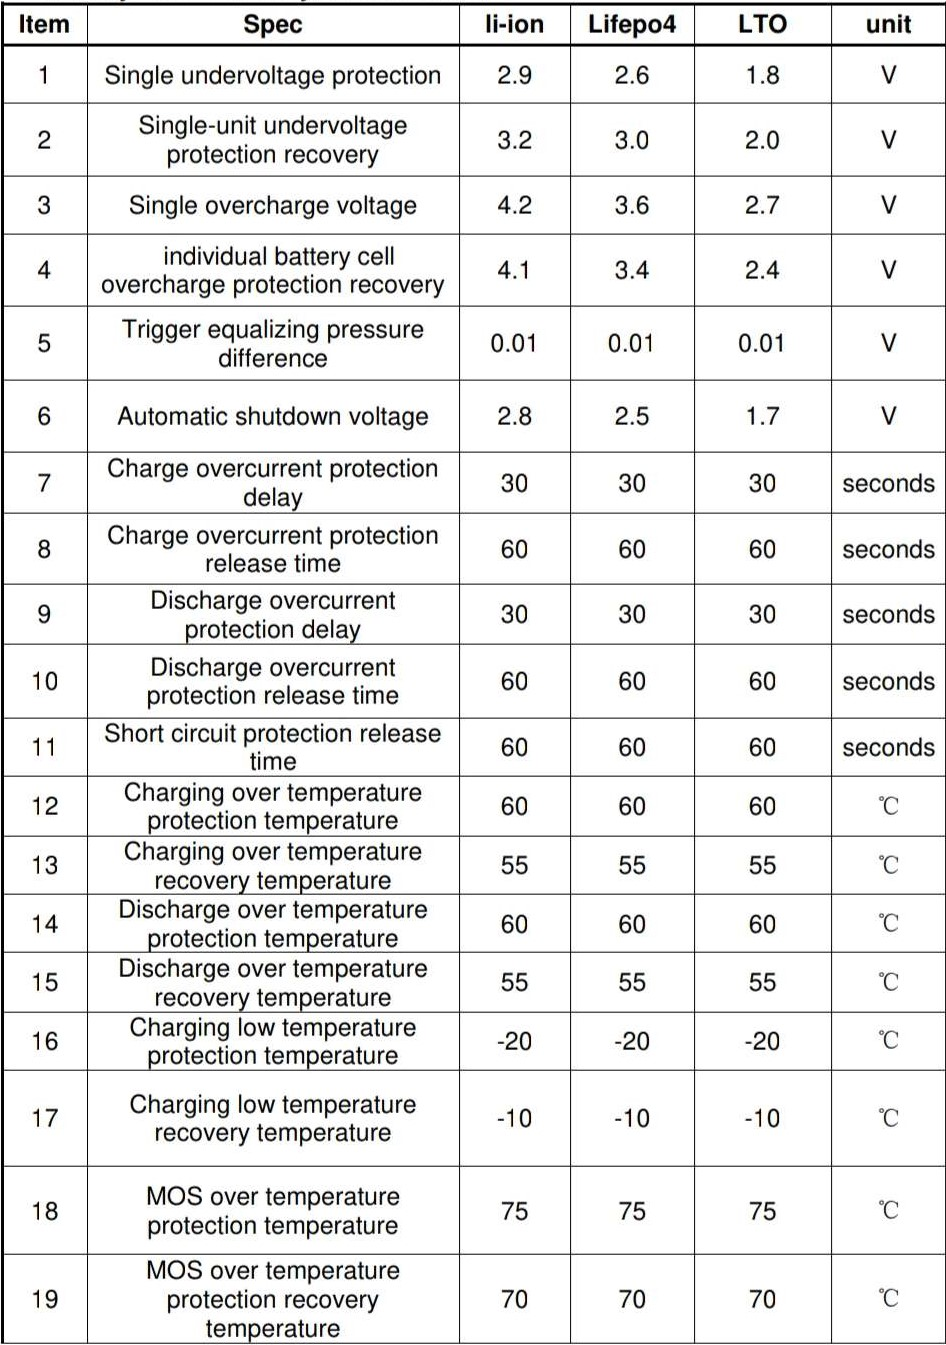
\includegraphics[width=0.5\linewidth]{Chapters/img/BMS_Setting.jpg}
		\centering
		\captionsetup{justification=centering,margin=2cm}
		\caption{ตารางการตั้งค่าตัวแปรของระบบการจัดการแบตเตอรี่ของโมดูลแบตเตอรี่ 72V30Ah}
		\label{fig:BMS_Setting}
	\end{figure}
	\begin{figure}[H]
		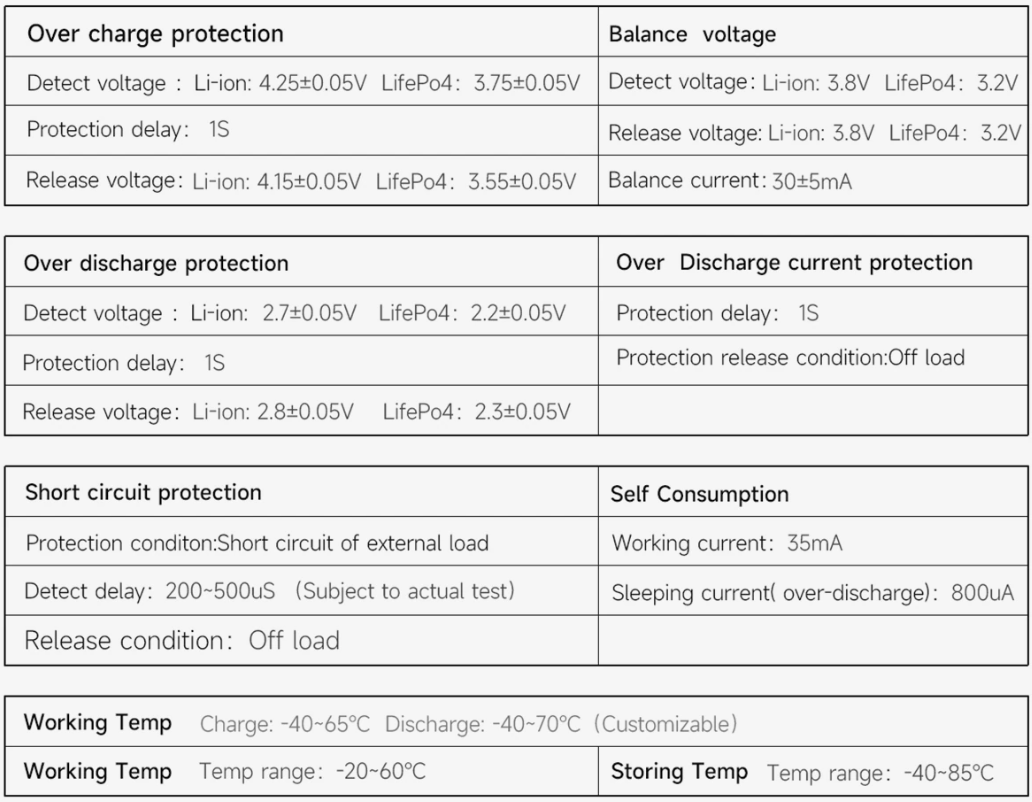
\includegraphics[width=1\linewidth]{Chapters/img/BMS_Setting2.PNG}
		\centering
		\captionsetup{justification=centering,margin=2cm}
		\caption{ตารางการตั้งค่าตัวแปรของระบบการจัดการแบตเตอรี่ของโมดูลแบตเตอรี่ 72V72Ah}
		\label{fig:BMS_Setting2}
	\end{figure}
\end{center}
%------------------------------------------------------------------------------------------
\chapter{คู่มือการใช้งานโปรแกรม Chroma 17020}
 เมื่อเปิดโปรแกรม Chroma 17020 จะพบกับหน้าเข้าสู่ระบบดังรูปที่\ref{fig:Loggin}
 \begin{center}
	\begin{figure}[H]
		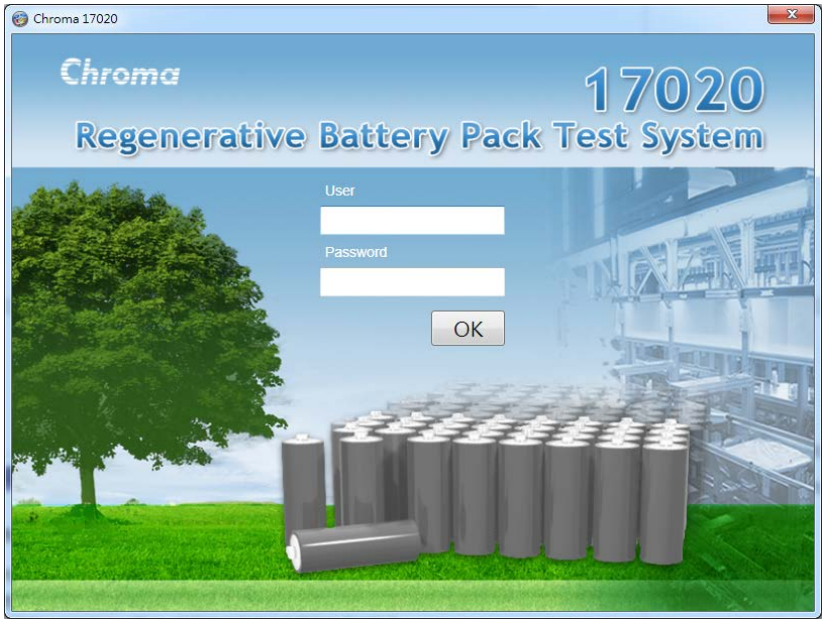
\includegraphics[width=1\linewidth]{Chapters/img/17020_Program/Loggin.png}
		\centering
		\captionsetup{justification=centering,margin=2cm}
		\caption{หน้าเข้าสู่ระบบ}
		\label{fig:Loggin}
	\end{figure}
\end{center}
โดยรหัสผ่านค่าเริ่มต้นจากโรงงานคือ User:root, Password:root เมื่อเข้าสู่ระบบได้แล้วจะพบกับหน้าต่างดังรูปที่\ref{Main_window}
\begin{center}
	\begin{figure}[H]
		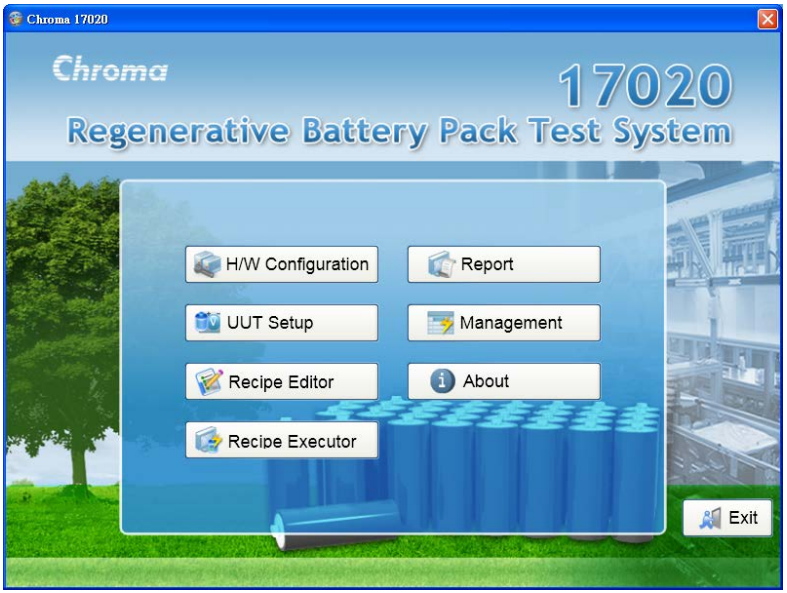
\includegraphics[width=1\linewidth]{Chapters/img/17020_Program/Home.png}
		\centering
		\captionsetup{justification=centering,margin=2cm}
		\caption{หน้าหลัก}
		\label{Main_window}
	\end{figure}
\end{center}
ซึ่งหน้านี้จะหน้าที่ใช้เพื่อเข้าสู่การตั้งค่าและการทำงานต่างๆของเครื่องทดสอบแบตเตอรี่ Chroma 17020 โดยจะประกอบไปด้วย 7 ส่วนดังนี้
\begin{itemize}
{\item H/W Configulation ในส่วนนี้คือส่วนสำหรับการเพิ่มอุปกรณ์วัดและทดสอบและ\\ตั้งค่าอุปกรณ์นั้นๆ}
{\item UUT Setup เป็นส่วนที่ใช้กำหนดขอบเขตของตัวแปรต่างๆ}
{\item Recipe Editor เป็นส่วนที่ตั้งค่าการทดสอบหรือใช้เพื่อกำหนดวิธีการทดสอบ}
{\item Recipe Executor เป็นส่วนที่ทำตามขั้นตอนการทดสอบที่ได้จาก Recipe Editor}
{\item Report เป็นส่วนที่ใช้รายงานผลการทดสอบ}
{\item Management เป็นส่วนที่ใช้สำหรับตั้งค่าอื่นๆในระบบเพิ่มเติม}
{\item About เป็นส่วนที่แสดงข้อมูลเบื้องต้นของระบบเช่น รุ่นของระบบ(Version) ผู้ใช้งาน(User)}
\end{itemize}
%**********************************************************************
\section{การตั้งค่าอุปกรณ์ในระบบ(Hardware Configuration)}
เมื่อเข้าสู่หน้าต่างในส่วนของ H/W Configulation จะพบกับหน้าต่างดังรูป
\begin{center}
	\begin{figure}[H]
		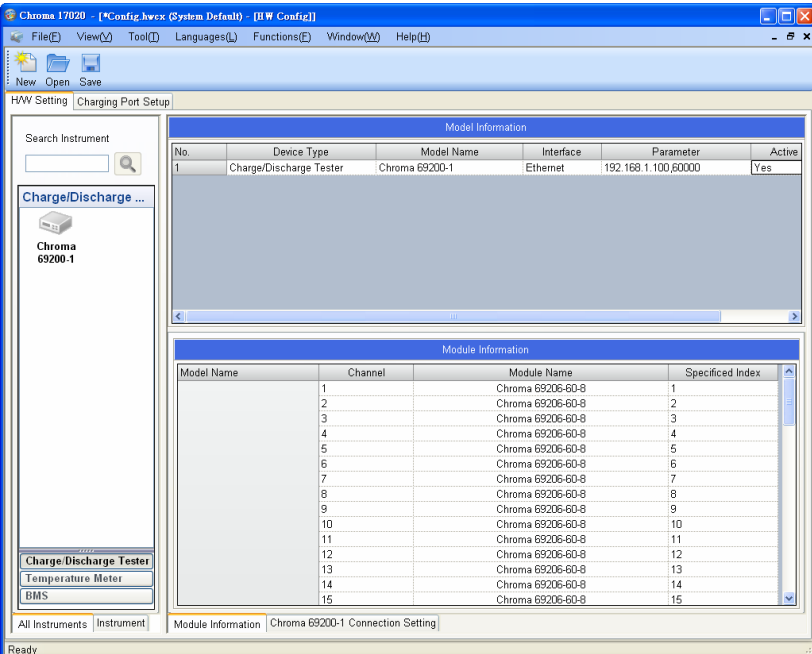
\includegraphics[width=1\linewidth]{Chapters/img/17020_Program/HW_Configulation/Main.png}
		\centering
		\captionsetup{justification=centering,margin=2cm}
		\caption{หน้าต่าง H/W Configulation}
	\end{figure}
\end{center}
โดยหน้าต่างนี้จะประกอบไปด้วย 3 ส่วนคือ
\begin{itemize}
{\item รายการเครื่องมือวัดที่สามารถใช้กับระบบนี้ได้}
{\item รายการเครื่องมือวัดที่เชื่อมต่อและการเชื่อมต่อ}
{\item การเลือกใช้งานเครื่องมือวัดต่อจำนวนอุปกรณ์ที่จะทำการวัด}
\end{itemize}
สำหรับการใช้งานเบื้องต้นถ้าหากต้องการสร้างการตั้งค่าขึ้นใหม่ให้กด file/new ตรงแถบเมนูด้านบนขวาของหน้าต่างนี้จากนั้นให้กด file/Auto Detect เพื่อให้ระบบค้นหาเครื่องมือวัดที่เชื่อมต่ออยู่ในระบบและตั้งค่าเครื่องมือวัดเบื้องต้นให้เองอัตโนมัติซึ่งถ้าหากตั้งค่าแล้วต้องทำการบันทึกข้อมูลทุกครั้งและถ้าหากต้องการใช้การตั้งค่านี้ให้กด file/Set As System Default
ในกรณีที่มีการบันทึกการตั้งค่าแล้วต้องการเรียกดูค่าการตั้งค่านั้นให้กด file/open แล้วเลือกดูการตั้งค่าตามที่ได้ตั้งชื่อไว้
%**********************************************************************
\subsection{ตั้งค่าข้อมูลเครื่องมือวัด(Setting Device Information)}
จากรูปที่ข.4 จะเป็นหน้าต่าง H/W Setting window ในหน้าจะสามารถตั้งค่าข้อมูลเครื่องมือวัดที่เชื่อมต่อเข้าสู่ระบบได้เช่น การเชื่อมต่อ(communication interface)และหมายเลขที่อยู่ไอพีของเครื่องมือวัด(IP Adress)
\newline
%++++++++++++++++++++++++++++++++++++++++++++++++
\newline
\textbf{การเพิ่มเครื่องมือวัดเข้าสู่ระบบ}
\newline \hspace*{2cm} 
การเพิ่มเครื่องมือวัดเข้าสู่ระบบให้จากรูปที่ข.4 คลิ๊กสองครั้งที่รูปเครื่องมือวัดหรือลากลงไปในหน้า All instuments หรือให้เข้าไปที่หน้า Instument คลิ๊กขวาที่จุดรวมเครื่องมือและเลือก Add Device 
ดังรูปที่ข.5 จากนั้นให้คลิ๊กขวาที่รูปเครื่องมือวัดแล้วเลือกเครื่องมือวัดที่ต้องการดังรูปที่ข.6 ซึ่งในตัวอย่างนี้จะเป็นการเลือกเครื่อง Chroma 69200-1 เข้าสู่ระบบจากนั้นเมื่อเลือกเสร็จหน้าต่างดังรูปที่ข.7 จะปรากฎให้กดตกลง
\begin{center}
	\begin{figure}[H]
		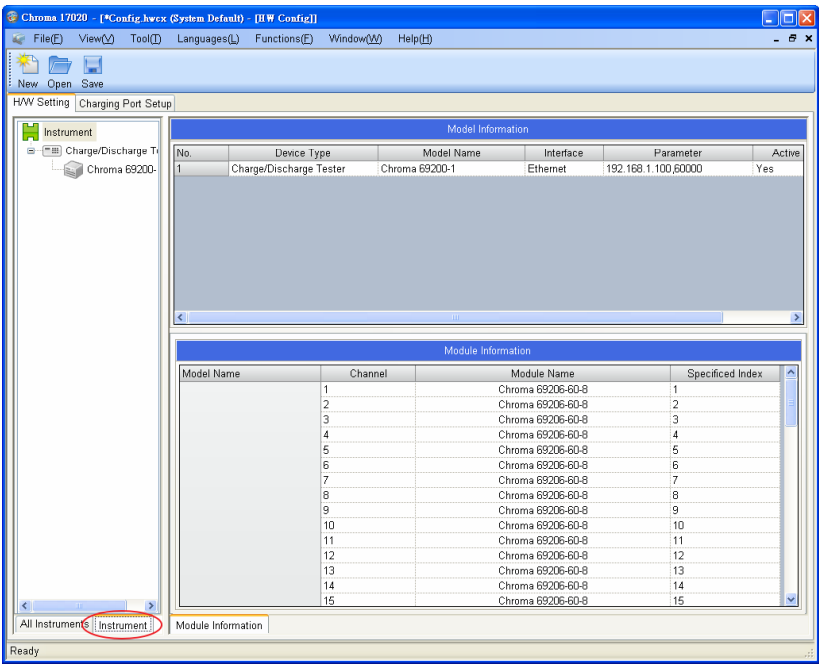
\includegraphics[width=1\linewidth]{Chapters/img/17020_Program/HW_Configulation/Device_Tree.png}
			\centering
			\captionsetup{justification=centering,margin=2cm}
			\caption{หน้า Instument}
	\end{figure}
	\begin{figure}[H]
		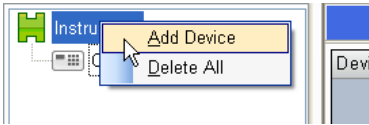
\includegraphics[width=1\linewidth]{Chapters/img/17020_Program/HW_Configulation/Adding_a_device.png}
			\centering
			\captionsetup{justification=centering,margin=2cm}
			\caption{การเพิ่มเครื่องมือวัด}
	\end{figure}
	\begin{figure}[H]
		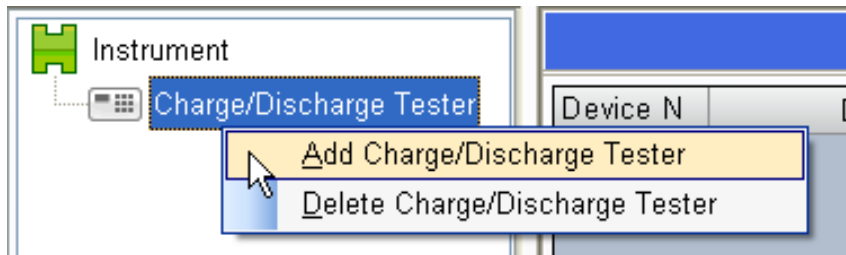
\includegraphics[width=1\linewidth]{Chapters/img/17020_Program/HW_Configulation/Adding_Charge.png}
			\centering
			\captionsetup{justification=centering,margin=2cm}
			\caption{การเพิ่ม Charge/Discharge Tester}
	\end{figure}
	\begin{figure}[H]
		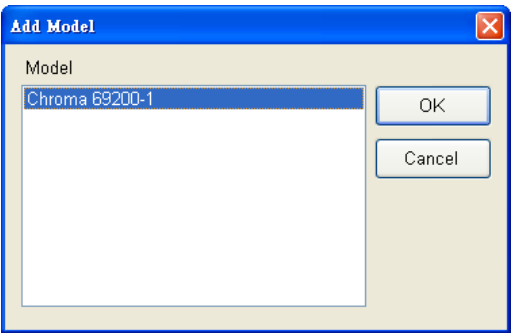
\includegraphics[width=1\linewidth]{Chapters/img/17020_Program/HW_Configulation/Add_Model.png}
			\centering
			\captionsetup{justification=centering,margin=2cm}
			\caption{เลือกรุ่นของเครื่องมือวัด}
	\end{figure}
\end{center}
%++++++++++++++++++++++++++++++++++++++++++++++++
\textbf{การตั้งค่าหมายเลขที่อยู่ไอพี(IP Adress)}
\newline \hspace*{2cm}
ในรูปที่ข.8 จะเป็นตารางข้อมูลการเชื่อมต่อของเครื่องมือวัดต่างๆที่เชื่อมต่ออยู่ในระบบซึ่งถ้าหากต้องการเปลี่ยนแปลงหมายเลยที่อยู่ไอพี(IP Adress)ให้คลิ๊กสองครั้งที่หมายเลขที่อยู่ไอพีที่ต้องการจะตั้งค่า
เมื่อคลิ๊กแล้วจะปรากฎหน้าต่างดังรูปที่ข.9 จากนั้นให้ตั้งค่าตามที่ต้องเมื่อตั้งค่าเสร็จให้กดตกลง
\begin{center}
	\begin{figure}[H]
		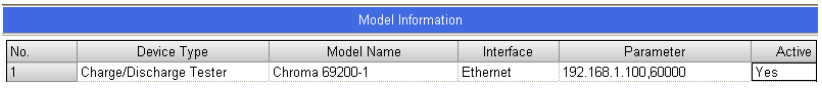
\includegraphics[width=1\linewidth]{Chapters/img/17020_Program/HW_Configulation/Model_info.png}
		\centering
		\captionsetup{justification=centering,margin=2cm}
		\caption{ข้อมูลการเชื่อมต่อของเครื่องมือวัด}
	\end{figure}
	\begin{figure}[H]
		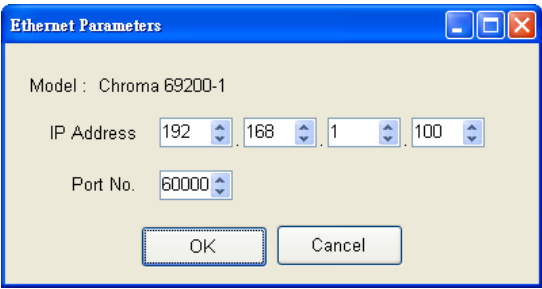
\includegraphics[width=1\linewidth]{Chapters/img/17020_Program/HW_Configulation/IP_Address.png}
		\centering
		\captionsetup{justification=centering,margin=2cm}
		\caption{หน้าต่างการตั้งค่าหมายเลขที่อยู่ไอพี}
	\end{figure}
\end{center}
%++++++++++++++++++++++++++++++++++++++++++++++++
\textbf{ทดสอบการเชื่อมต่อของเครื่องมือวัด(Connection Test)}
\newline \hspace*{2cm}
เมื่อทำการตั้งค่าอุปกรณ์แล้วทำการบันทึกข้อมูลเรียบร้อยแล้วให้ทำการทดสอบการเชื่อมต่อของเครื่องมือวัดโดยให้เข้าไปที่ file/Connection Test แล้วหน้าต่างการทดสอบการเชื่อมต่อจะปรากฎดังรูปที่ข.10
ซึ่งในรูปจะเห็นว่าการทดสอบการเชื่อมต่อของเครื่องมือวัดนั้นเสร็จสิ้นโดยไม่มีข้อผิดพลาด
\begin{center}
	\begin{figure}[H]
		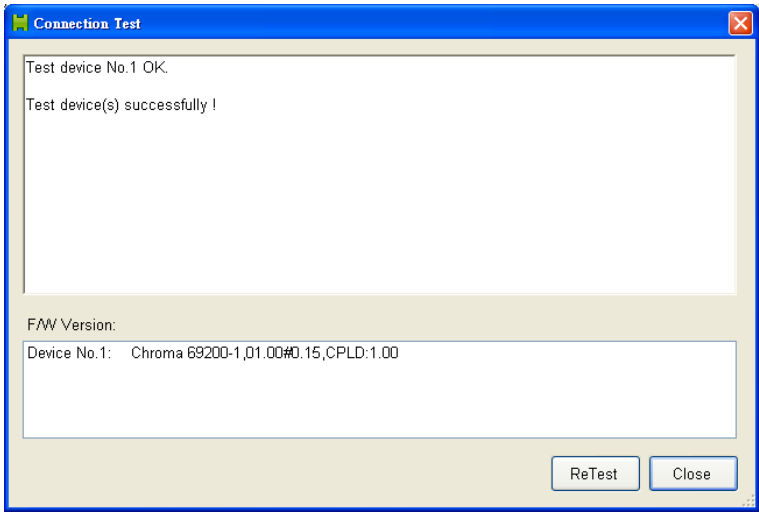
\includegraphics[width=1\linewidth]{Chapters/img/17020_Program/HW_Configulation/Connection_test.png}
		\centering
		\captionsetup{justification=centering,margin=2cm}
		\caption{ข้อมูลการเชื่อมต่อของเครื่องมือวัด}
	\end{figure}
\end{center}
%**********************************************************************
\section{การตั้งค่าขอบเขตตัวแปรต่างๆ(UUT Setup)}
จากหน้าต่างแรกให้คลิ๊กที่ UUT Setup จากนั้นหน้าต่าง UUT Setup จะปรากฎดังรูปที่ข.11 ในหน้านี้เราสามารถตั้งค่าขอบเขตของตัวแปรต่างๆให้เหมาะสมกับการทดสอบแบตเตอรี่ได้เพื่อป้องกันไม่ให้เครื่องอัดและคายประจุ
นั้นอัดประจุหรือคายประจุเกินกว่าที่ได้กำหนดหรือสำหรับอุปกรณ์อื่นก็จะไม่สามารถทำงานเกินกว่าขอบเขตตามที่ได้ตั้งค่าไว้ในหน้าต่างนี้และเมื่อทำการตั้งค่าเสร็จแล้วให้ทำการบันทึกข้อมูล
\begin{center}
	\begin{figure}[H]
		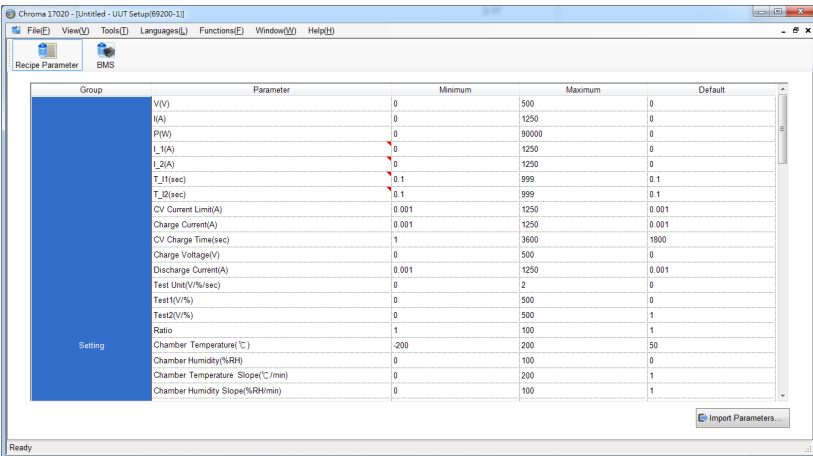
\includegraphics[width=1\linewidth]{Chapters/img/17020_Program/UUT/UUT_setup_win.png}
		\centering
		\captionsetup{justification=centering,margin=2cm}
		\caption{หน้าต่าง UUT Setup}
	\end{figure}
\end{center}
%**********************************************************************
\section{การตั้งค่าการทดสอบหรือวิธีขั้นตอนการทดสอบ(Recipe Editor)}
จากหน้าต่างแรกให้คลิ๊กที่ Recipe Editor จากนั้นหน้าต่าง Recipe Editor จะปรากฎดังรูปที่ข.12 ซึ่งในหน้าต่างนี้จะเป็นหน้าสำคัญที่เอาไว้ใช้กำหนดขั้นตอนการทดสอบและตัวแปรต่างๆสำหรับการทดสอบ
โดยเมื่อได้เข้ามาสู่หน้าต่างนี้ถ้าหากมีข้อมูลที่ได้ทำการบันทึกไว้ก่อนหน้านี้แล้วต้องการจะเรียกข้อมูลให้เลือก Open จากนั้นให้เลือกข้อมูลที่ได้ทำหารบันทึกไว้ก่อนหน้าและกดตกลงดังรูปที่ข.13
ถ้าหาต้องการจะสร้างใหม่ให้เลือก New และกดตกลง
\begin{center}
	\begin{figure}[H]
		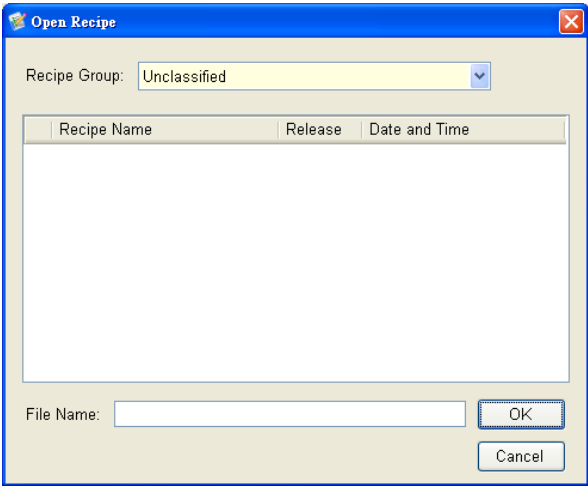
\includegraphics[width=1\linewidth]{Chapters/img/17020_Program/Recipe_Editor/Recipe_dialog.png}
		\centering
		\captionsetup{justification=centering,margin=2cm}
		\caption{หน้าต่างแรกเมื่อเข้าสู่ Recipe Editor}
	\end{figure}
	\begin{figure}[H]
		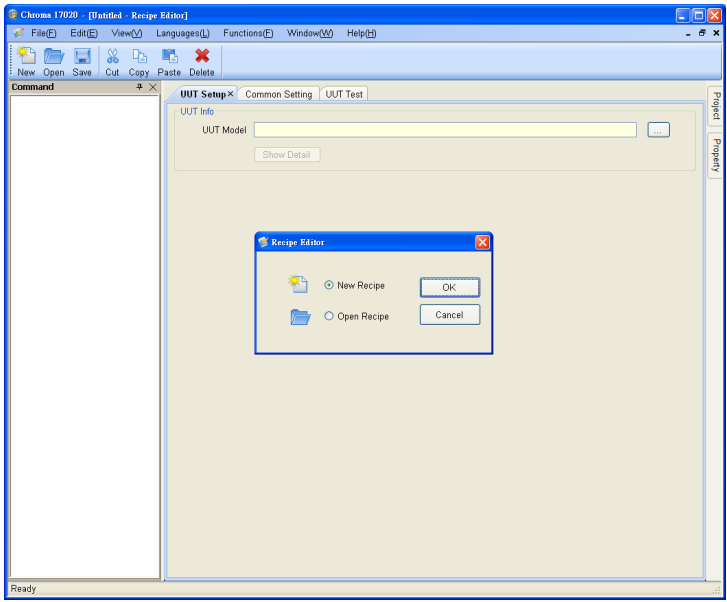
\includegraphics[width=1\linewidth]{Chapters/img/17020_Program/Recipe_Editor/Recipe_editor_win.png}
		\centering
		\captionsetup{justification=centering,margin=2cm}
		\caption{หน้าต่างเลือกข้อมูลการตั้งค่าอื่นๆ}
	\end{figure}
\end{center}
ซึ่งไม่ว่าจะเลือกข้อมูลที่ได้มีการตั้งค่าอยู่แล้วหรือจะสร้างการตั้งค่าใหม่ก็จะเข้าสู่หน้าถัดไปดังรูปข.14 ซึ่งสำหรับการสร้างการตั้งค่าใหม่ให้ทำการเลือกขอบเขตตัวแปรที่ได้จากการตั้งค่าใน UUT Setup ดังกรอบสีแดงดังรูปเมื่อเลือกเสร็จ
ให้กดตกลง และจะเห็นได้ว่าหน้าต่างนี้จะมีแถบหน้าต่างอยู่ทั้งสิ้น 5 ส่วนดังนี้คือ UUT Setup, Common Setting, UUT Test, Protection และ Remote Alarm
\begin{center}
	\begin{figure}[H]
		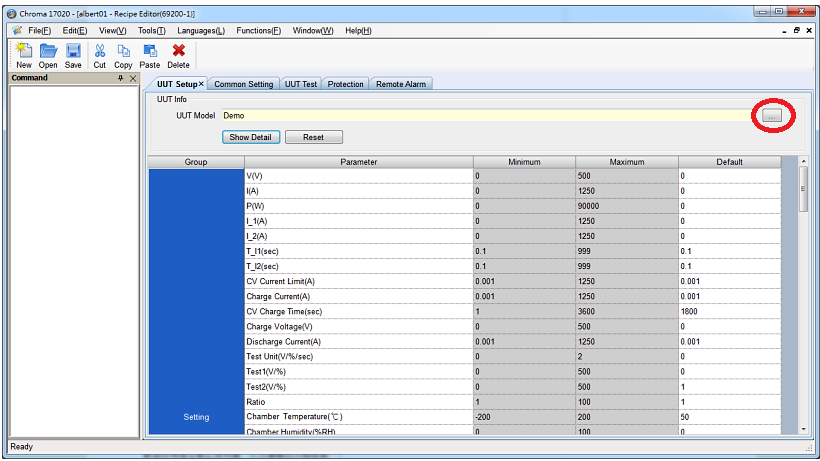
\includegraphics[width=1\linewidth]{Chapters/img/17020_Program/Recipe_Editor/Setting_param_UUT_recipe_editor.png}
		\centering
		\captionsetup{justification=centering,margin=2cm}
		\caption{หน้าต่างแรกเมื่อเข้าสู่ Recipe Editor}
	\end{figure}
\end{center}
%++++++++++++++++++++++++++++++++++++++++++++++++
\textbf{การตั้งค่าการแจ้งเตือน(Remote Alarm)}
\newline \hspace*{2cm}
ในหน้าต่างนี้จะสามารถตั้งค่าการแจ้งเตือนต่างๆได้เมื่อเครื่องมือวัดสมารถตรวจสอบความผิดพลาดหรือค่าตัวแปรต่างๆนั้นเกินขอบเขตที่ได้กำหนดไว้ดังหัวข้อต่างๆถ้าหากต้องการให้มีการแจ้งเตือน
ให้คลิ๊กที่กล่องสี่เหลี่ยมหน้าหัวข้อที่ต้องการให้มีการเเจ้งเตือนดังรูปที่ข.15
\begin{center}
	\begin{figure}[H]
		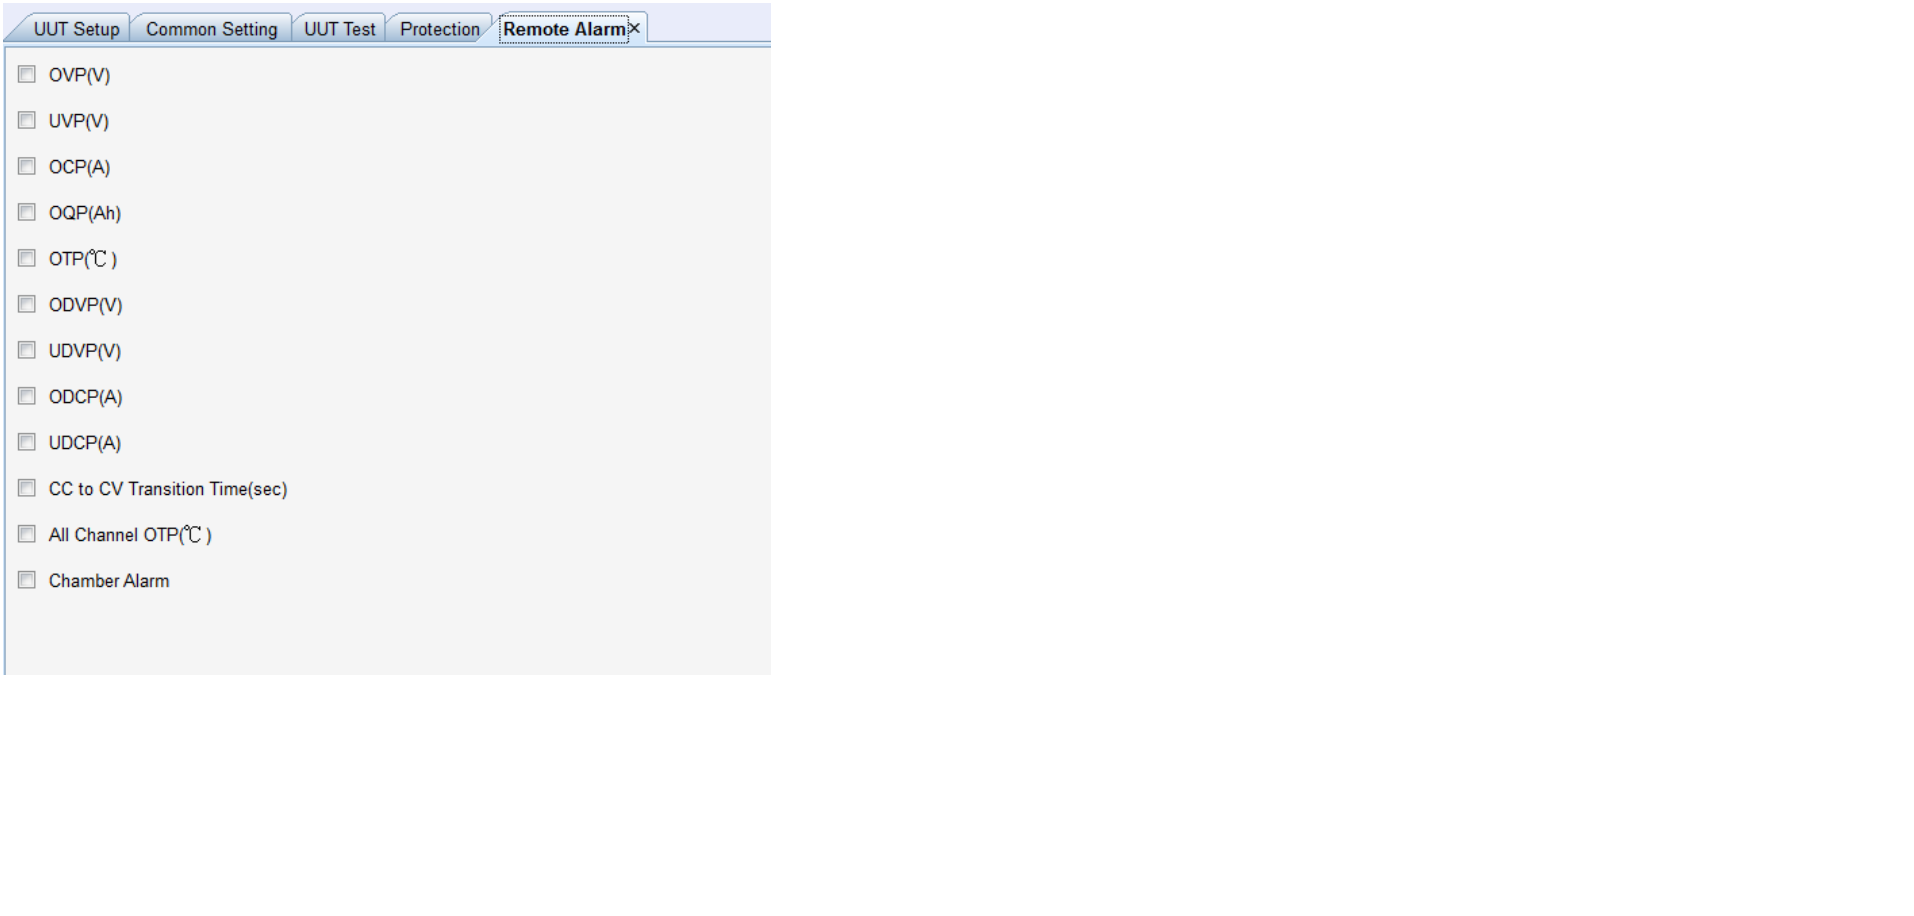
\includegraphics[width=1\linewidth]{Chapters/img/17020_Program/Recipe_Editor/setting_remote_alarm.png}
		\centering
		\captionsetup{justification=centering,margin=2cm}
		\caption{หน้าต่าง Remote Alarm}
	\end{figure}
\end{center}
%++++++++++++++++++++++++++++++++++++++++++++++++
\textbf{การตั้งค่าการป้องกัน(Protection)}
\newline \hspace*{2cm}
ในหน้าต่างนี้จะสามารถตั้งค่าเงื่อนไขการป้องกันในตัวแปรต่างๆได้คล้ายกับการตั้งค่าขอบเขตในหน้าต่าง UUT Setup ซึ่งความแตกต่างระหว่างการตั้งค่าทั้ง 2 นี้คือสำหรับการตั้งค่าขอบเขตนั้นจะเป็นการกำหนดขอบเขตเพื่อไม่ให้
ทำการตั้งค่าอื่นๆในหน้าต่างอื่นๆนั้นจะไม่สามารถตั้งค่าได้เกินขอบเขตที่ได้กำหนดไว้ได้แต่สำหรับการตั้งค่าการป้องกันนั้นจะเป็นการกำหนดเงื่อนไขที่จะทำให้ระบบเครื่องมือวัดของเครื่อง Chroma 17020 นั้นจะทำการหยุดการทดสอบเพื่อ
ป้องกันความเสียหายที่จะเกิดขึ้นกับแบตเตอรี่หรือความเสียหายที่จะเกิดขึ้นกับเครื่องมือวัดได้โดยการตั้งค่าเงื่อนไขในตัวแปรต่างๆจะสามารถตั้งค่าได้ดังรูปที่ข.16
\begin{center}
	\begin{figure}[H]
		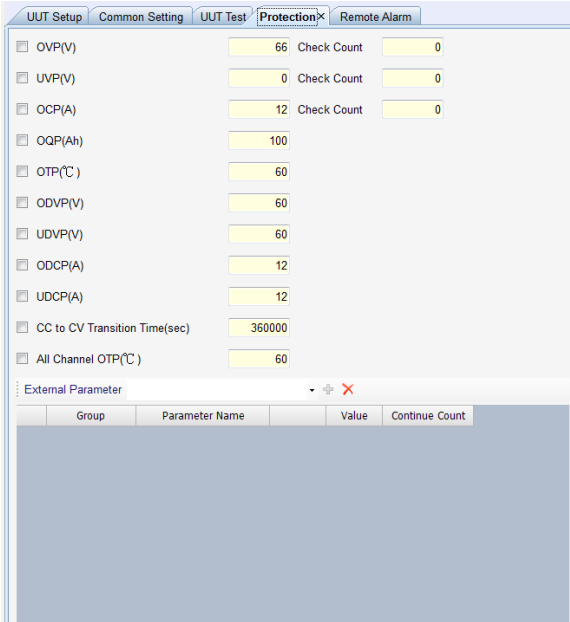
\includegraphics[width=1\linewidth]{Chapters/img/17020_Program/Recipe_Editor/setting_protection.png}
		\centering
		\captionsetup{justification=centering,margin=2cm}
		\caption{หน้าต่าง Protection}
	\end{figure}
\end{center}
%++++++++++++++++++++++++++++++++++++++++++++++++
\textbf{การตั้งค่าขั้นตอนการทดสอบ(UUT Test)}
\newline \hspace*{2cm}
สำหรับหน้าต่างนี้จะเป็นหน้าต่างที่มีความสำคัญลำดับต้นๆเนื่องจากหน้าต่างนี้จะใช้สำหรับในการตั้งค่าการกำหนดขั้นตอนการทดสอบแบตเตอรี่ของระบบเช่น การอัดประจุ การคายประจุ เป็นต้นโดยหน้าต่างนี้จะมีลักษณะดังรูปที่ข.17
ซึ่งจะประกอบไปด้วย 3 ส่วนหลักคือ 
\begin{itemize}
{\item คำสั่งต่างๆที่ใช้สำหรับการทดสอบ}
{\item ลำดับขั้นตอนของคำสั่งในการทดสอบ}
{\item การตั้งค่าเพิ่มเติม}
\end{itemize}
\begin{center}
	\begin{figure}[H]
		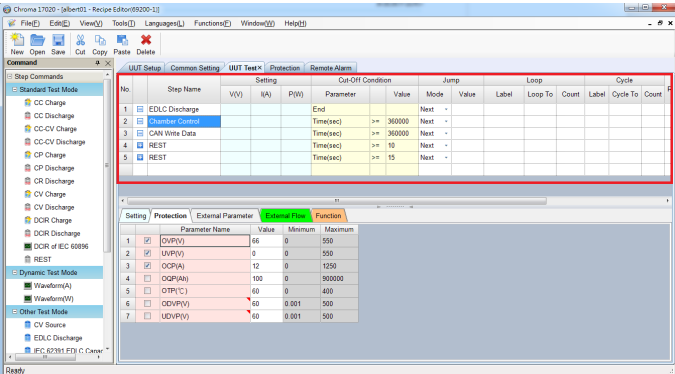
\includegraphics[width=1\linewidth]{Chapters/img/17020_Program/Recipe_Editor/UUT_tesing_page.png}
		\centering
		\captionsetup{justification=centering,margin=2cm}
		\caption{หน้าต่าง Protection}
	\end{figure}
\end{center}
โดยในส่วนลำดับขั้นตอนของคำสั่งซึ่งคำสั่งต่างๆจะถูกจัดลำดับการทำงานเป็นตารางซึ่งในการเพิ่มคำสั่งให้คลิ๊กที่ตารางแล้วจากนั้นให้คลิ๊ก 2 ครั้งที่คำสั่งที่ต้องการจะเพิ่มแล้วคำสั่งจะถูกเพิ่มเข้ามาอยู่ในตารางในกรณีที่ต้องการเพิ่มคำสั่งที่
เหมือนกับคำสั่งก่อนหน้าให้คลิ๊กที่คำสั่งที่ต้องการคัดลอกแล้วกดคัดลอก(Copy)ตรงแถบด้านบนดังรูปที่ข.17 จากนั้นให้กดวาง(Past)ที่ตารางลำดับคำสั่งแล้วคำสั่งที่ได้ทำการคัดลอกจะมาปรากฎอยู่ในตารางซึ่งตัวแปรต่างๆ
ที่ได้ทำการตั้งค่าไว้แล้วก่อนหน้าเมื่อกดวางแล้วคำสั่งใหม่ที่ถูกเพิ่มเข้ามานั้นจะมีการตั้งค่าที่เหมือนกันทุกประการหากต้องการที่จะลบคำสั่งให้คลิ๊กที่คำสั่งหนึ่งครั้งแล้วกดลบ(Delete) 
\newline \hspace*{2cm}
สำหรับส่วนประกอบต่างๆในตารางลำดับคำสั่งโดยเรียงลำดับจากซ้ายไปขวาจะมีดังนี้
\begin{itemize}
{\item (No.) ลำดับคำสั่ง}
{\item (Step Name) ชื่อคำสั่ง}
{\item (Setting) ค่าตัวแปรสำหรับคำสั่งคือ แรงดันไฟฟ้าV(V) กระแสไฟฟ้าI(A) กำลังไฟฟ้าP(W) โดยในส่วนนี้สามารถกำหนดค่าได้}
{\item (Cut-Off Condition) เงื่อนไขการสิ้นสุดคำสั่งนั้นๆ}
{\item (Jump) ขั้นตอนการทำงานถัดไปเมื่อสิ้นสุดคำสั่งนั้นๆโดยสามารถเลือกได้ดังนี้คือ ทำคำสั่งถัดไปในตาราง(Next),\newline สิ้นสุดการทำงาน(End), 
ข้ามไปทำคำสั่งที่ได้ตั้งค่าไว้(Jump to Step),พักชั่วคราวตามที่ได้ตั้งค่าไว้ในหน่วยวินาที(Rest),ทำตามเงื่อนไข(If)และ}
{\item (Loop) กำหนดการทำคำสั่งซ้ำ (Label)เป็นคอลัมน์ที่ใช้เพื่อกำหนดคำสั่งที่ต้องการทำซ้ำ (Loop to)เป็นคอลัมน์ที่ใช้เพื่อกำหนดคำสั่งที่ต้องการทำซ้ำไปถึงคำสั่งที่มีการกำหนด\newline
	    (Count) กำหนดจำนวนครั้งที่ต้องการทำซ้ำ}
\end{itemize}
%************************************************************************************************************
\section{การสั่งการทำงานตามขั้นตอนการทดสอบ(Recipe Executor)}
คลิ๊กที่เมนู Recipe Executor จากหน้าต่างหลักเพื่อเข้าสู่หน้าต่างการทำงานนี้ดังในรูป\ref{fig:main_Recipe_Executor}ซึ่งในรูปจะแสดงช่องทางการทดสอบแบตเตอรี่ที่สามารถใช้ในการทดสอบได้
ทั้งหมด
\begin{center}
	\begin{figure}[H]
		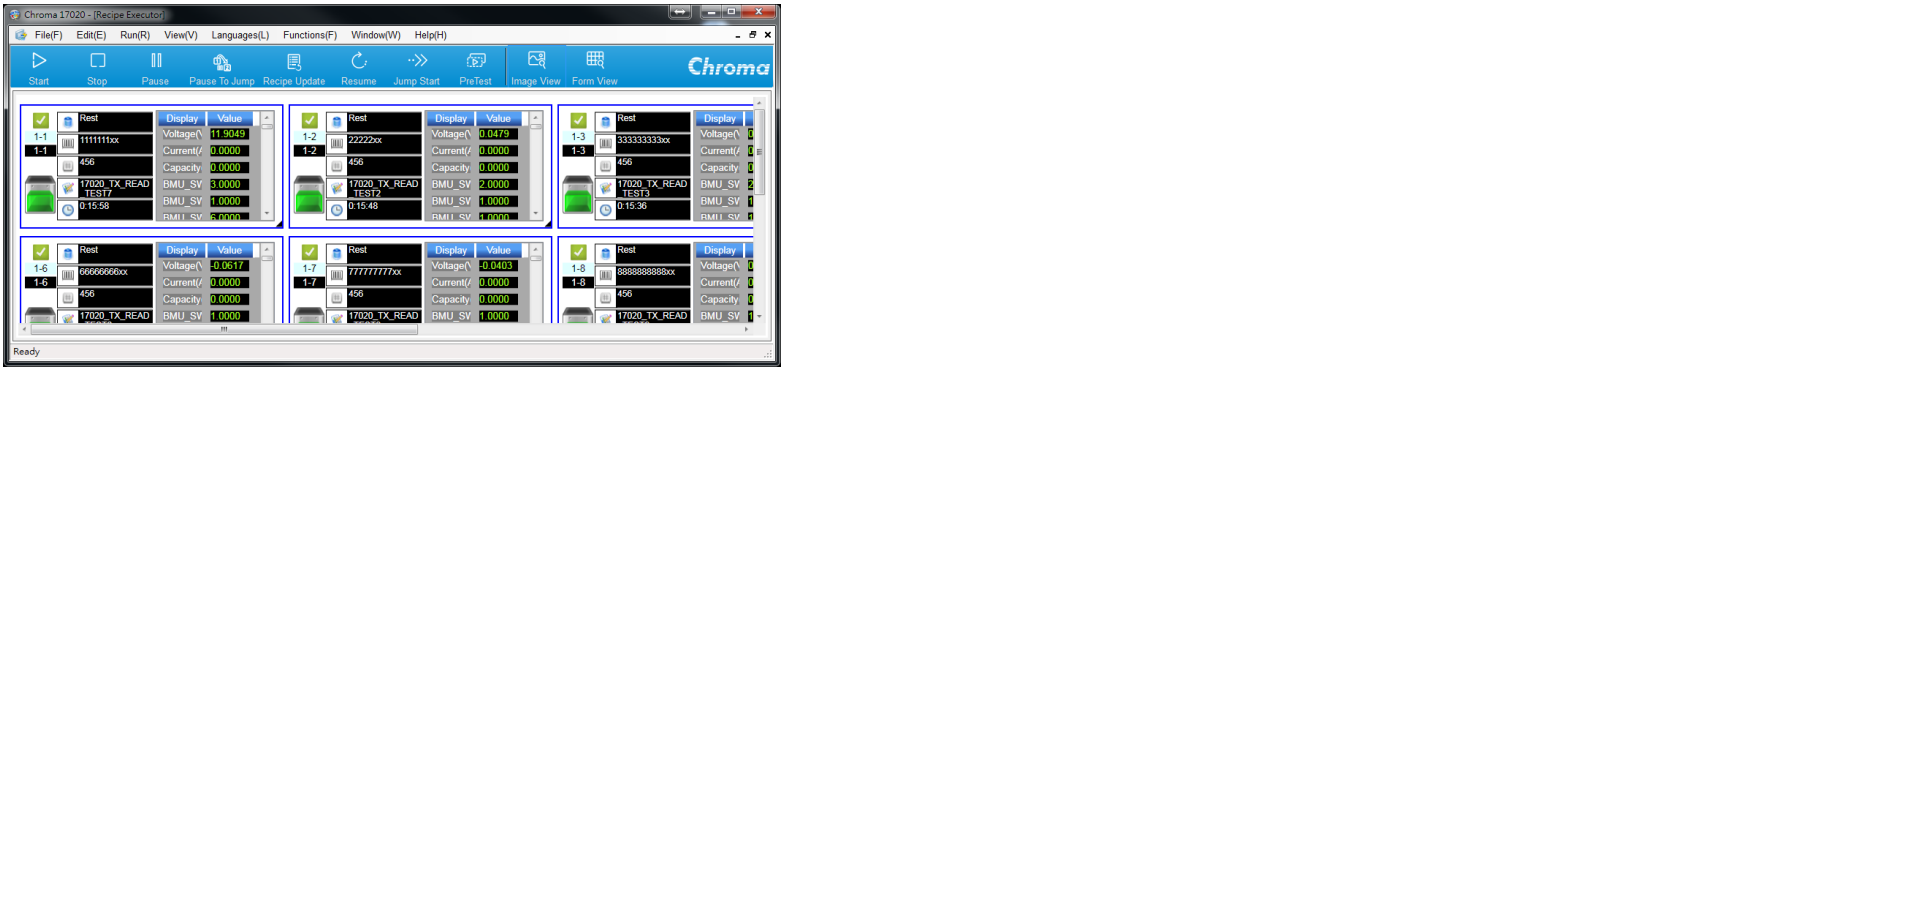
\includegraphics[width=1\linewidth]{Chapters/img/17020_Program/Recipe_Executor/Recipe_executor_main_win.png}
		\centering
		\captionsetup{justification=centering,margin=2cm}
		\caption{หน้าต่างหลัก Recipe Executor}
		\label{fig:main_Recipe_Executor}
	\end{figure}
\end{center}
ในการเลือกช่องทางในการทดสอบแบตเตอรี่ที่ต้องการสามารถกดเลือกช่องสี่เหลี่ยมตรงช่องทางที่ต้องการดังรูปที่\ref{fig:select_box} จากนั้นให้ทำการเลือกขั้นตอนการทดสอบที่ได้ทำการตั้งค่าไว้แล้วดังรูปที่\ref{fig:data_display_recipe_executor} ในกรณีที่ไม่มีรูป(Icon)แสดงขึ้นมาดังในวงกลมสีแดงให้ทำการกดที่คำว่า Recipe Name แทนเมื่อคลิ๊กเข้าไปแล้วจะพบกับหน้าต่างดังรูปที่\ref{fig:recipe_setup_win}ให้ทำการเลือกชื่อลำดับขั้นตอนที่ได้ตั้งค่าไว้แล้วจากเมนู Recipe Editor โดยเลือกขั้นตอนที่ต้องการ
ให้ตรงกับช่องทางการทดสอบที่ต้องการจากนั้นให้กดตกลงจากนั้นให้กด Start จากเมนูด้านบนในรูปที่\ref{fig:main_Recipe_Executor}หลังจากที่ได้เริ่มทำการทดสอบแล้วโดยถ้าหากต้องการดูข้อมูลการทดสอบ
ให้กดที่รูปกล่องสีเขียวจากนั้นกราฟข้อมูลการทดสอบจะปรากฎขึ้นดังรูปที่\ref{fig:ch_graph}

\begin{center}
	\begin{figure}[H]
		\centering
		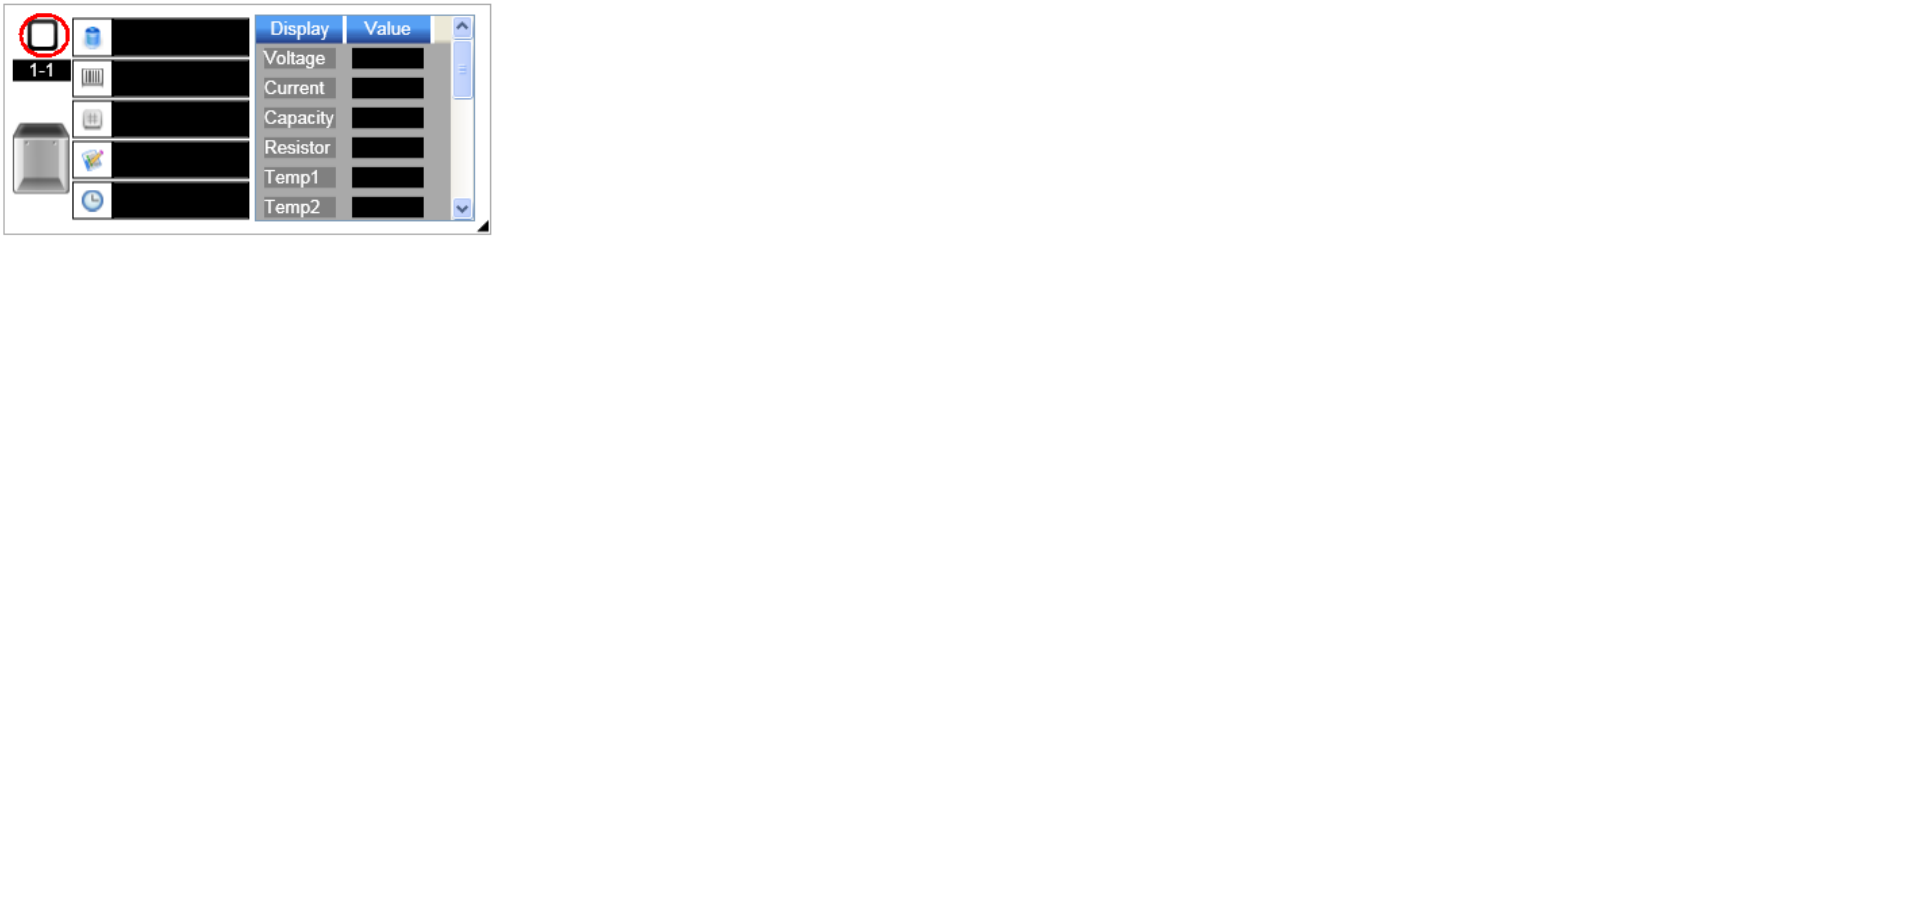
\includegraphics[width=1\linewidth]{Chapters/img/17020_Program/Recipe_Executor/battery_select_box.png}
		\centering
		\captionsetup{justification=centering,margin=2cm}
		\caption{เลือกช่องทางการทดสอบ}
		\label{fig:select_box}
	\end{figure}
	\begin{figure}[H]
		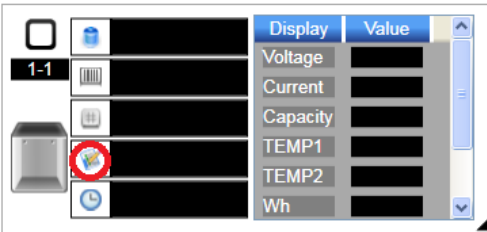
\includegraphics[width=1\linewidth]{Chapters/img/17020_Program/Recipe_Executor/battery_data_display.png}
		\centering
		\captionsetup{justification=centering,margin=2cm}
		\caption{เลือกขั้นตอนการทดสอบ (ก.)}
		\label{fig:data_display_recipe_executor}
	\end{figure}
	\begin{figure}[H]
		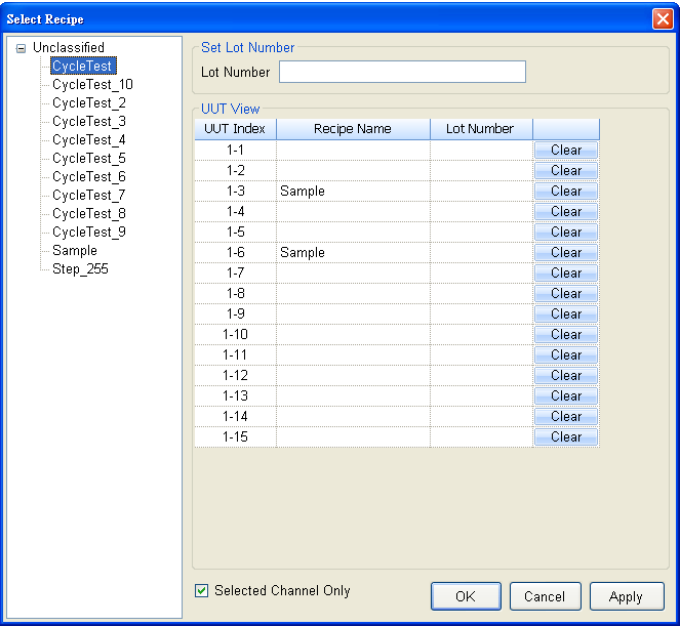
\includegraphics[width=1\linewidth]{Chapters/img/17020_Program/Recipe_Executor/recipe_setup_win.png}
		\centering
		\captionsetup{justification=centering,margin=2cm}
		\caption{เลือกขั้นตอนการทดสอบ (ข.)}
		\label{fig:recipe_setup_win}
	\end{figure}
	\begin{figure}[H]
		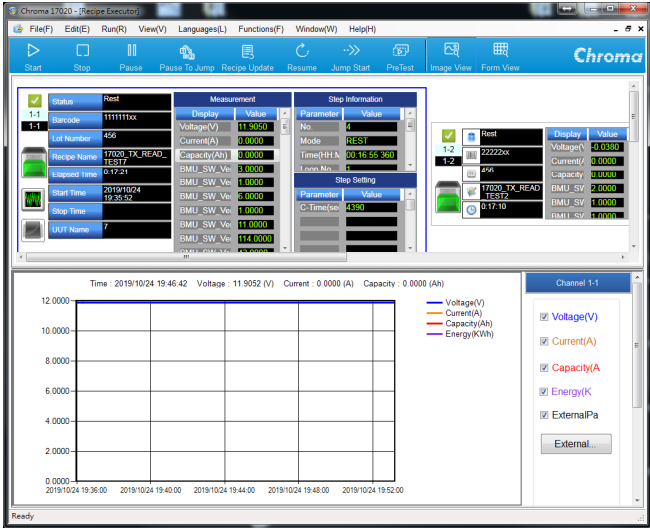
\includegraphics[width=1\linewidth]{Chapters/img/17020_Program/Recipe_Executor/ch_graph.png}
		\centering
		\captionsetup{justification=centering,margin=2cm}
		\caption{กราฟข้อมูลระหว่างการทดสอบ}
		\label{fig:ch_graph}
	\end{figure}
\end{center}
%************************************************************************************************************
\section{การแสดงผลข้อมูลที่ได้จากการทดสอบ(Report)}
กดเข้าเมนู Report จากในหน้าต่างหลักเพื่อเข้าสู่เมนูนี้แล้วหน้าต่างเมนู Report จะปรากฎดังรูปที่\ref{fig:report}จากนั้นให้เลือกข้อมูลที่ต้องการแสดงผลโดยกดเลือกที่ Generate เมื่อกดเข้าไปแล้ว
หน้าต่างเลือกข้อมูลจะปรากฏดังรูปที่\ref{fig:Selecting_data_data_analysis} จากนั้นให้ทำการเลือกข้อมูลเมื่อเลือกข้อมูลที่ต้องการแล้วให้กดตกลงจากนั้นให้กด Export to PDF
ตรงแถบเมนูด้านบนซึ่งข้อมูลที่ได้นี้จะเป็นข้อมูลอย่างคร่าวๆ
\begin{center}
	\begin{figure}[H]
		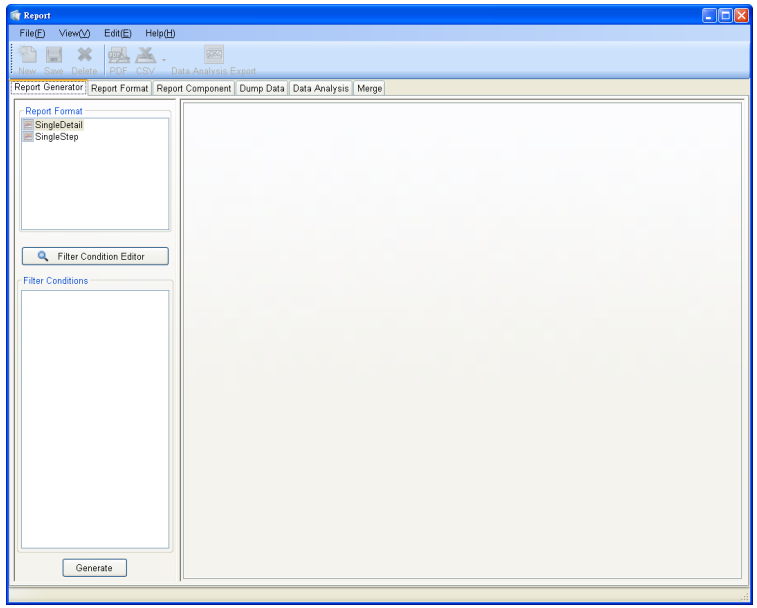
\includegraphics[width=1\linewidth]{Chapters/img/17020_Program/Report/Report_main_menu.png}
		\centering
		\captionsetup{justification=centering,margin=2cm}
		\caption{หน้าต่างหลักของเมนู Report}
		\label{fig:report}
	\end{figure}
	\begin{figure}[H]
		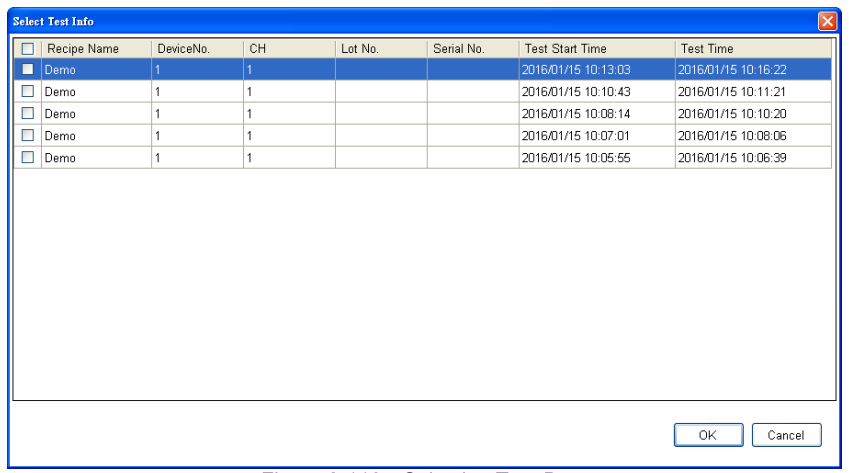
\includegraphics[width=1\linewidth]{Chapters/img/17020_Program/Report/Selecting_data.png}
		\centering
		\captionsetup{justification=centering,margin=2cm}
		\caption{หน้าต่างหลักของเมนู Report}
		\label{fig:Selecting_data_data_analysis}
	\end{figure}
\end{center}
โดยการนำข้อมูลการทดสอบอย่างละเอียดให้กดที่เมนู Data Analysis ที่แถบเมนูด้านบนแล้วหน้าต่างจะปรากฎขึ้นดังรูปที่\ref{fig:Data_analysis}โดยในหน้าต่างนี้จะเห็นได้ว่าด้านล่างของหน้าต่าง
จะมีให้กำหนดตัวแปรและแกนที่ต้องการจะวาดกราฟข้อมูลการทดสอบเมื่อกำหนดตัวแปรตามที่ต้องการแล้วให้กดเลือกข้อมูลที่ต้องการที่แถบเมนู Data Selection โดยต้องเลือกให้ตรงกับตัวแปรและแกนที่ได้กำหนดไว้แล้ว
จากนั้นเมื่อเลือกข้อมูลที่ต้องการได้แล้วให้ทำการกด Preview โปรแกรมจะทำการวาดกราฟข้อมูลการทดสอบตามข้อมูลที่ได้เลือกไว้จากนั้นให้กดเลือกเมนู Data เพื่อตรวจสอบความถูกต้องของข้อมูลการทดสอบโดยข้อมูลจะถูกแสดงผล
ออกมาในรูปแบบตารางดังรูปที่\ref{fig:Data_analysis_preview}เมื่อตรวจสอบความถูกต้องของข้อมูลการทดสอบที่ต้องการจะนำไปวิเคราะห์แล้วให้ทำการกดบันทึกข้อมูลโดยเลือกที่เมนู Data Analysis
Export จากนั้นหน้าต่างบันทึกข้อมูลจะปรากฎดังรูปที่\ref{fig:Export_data_analysis} จากนั้นให้ทำการตั้งชื่อและเลือกที่อยู่ของข้อมูลที่ต้องการบันทึกจากนั้นให้กดตกลง

\begin{center}
	\begin{figure}[H]
		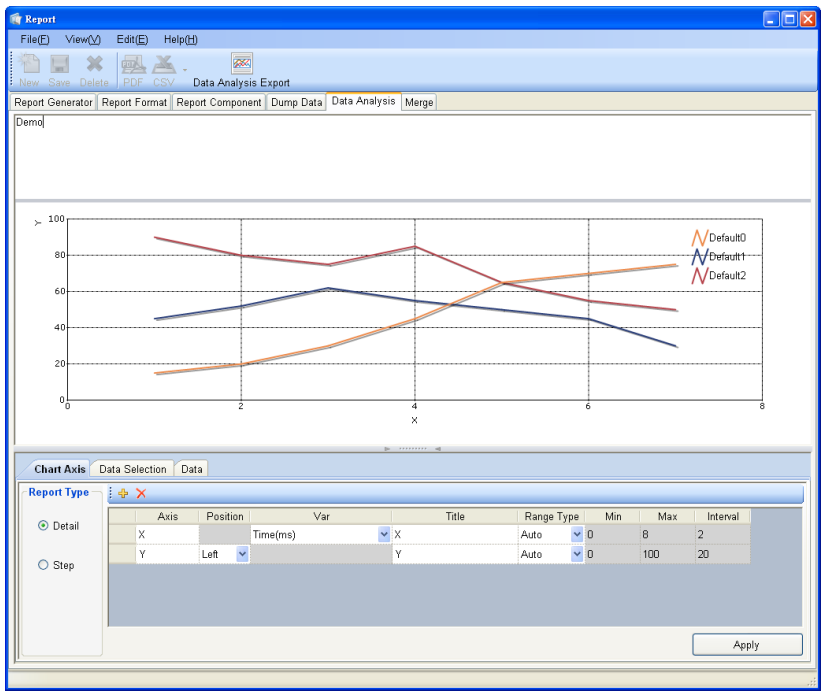
\includegraphics[width=1\linewidth]{Chapters/img/17020_Program/Report/Data_analysis.png}
		\centering
		\captionsetup{justification=centering,margin=2cm}
		\caption{หน้าต่างเมนู Data Analysis}
		\label{fig:Data_analysis}
	\end{figure}
	\begin{figure}[H]
		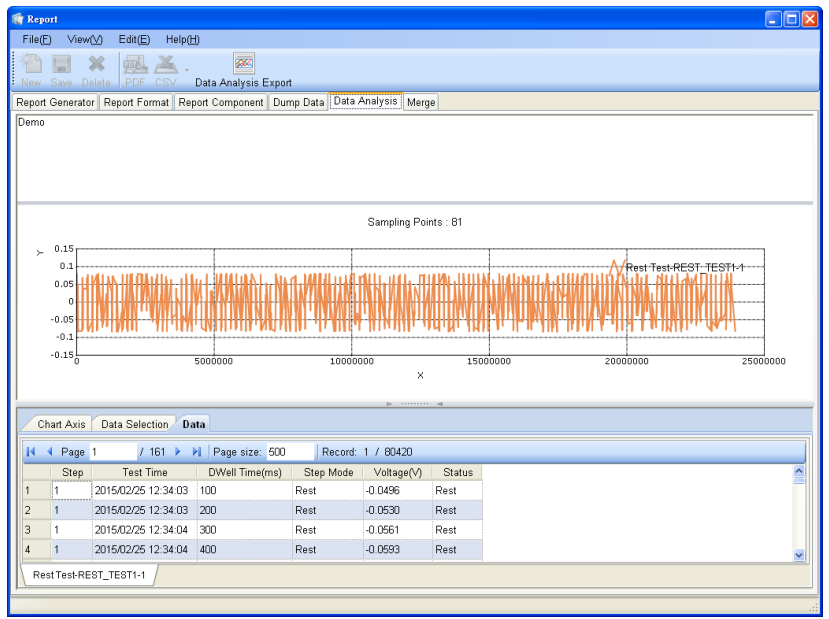
\includegraphics[width=1\linewidth]{Chapters/img/17020_Program/Report/Data_analysis_preview.png}
		\centering
		\captionsetup{justification=centering,margin=2cm}
		\caption{กราฟข้อมูลการทดสอบโดยเมนู Data Analysis}
		\label{fig:Data_analysis_preview}
	\end{figure}
	\begin{figure}[H]
		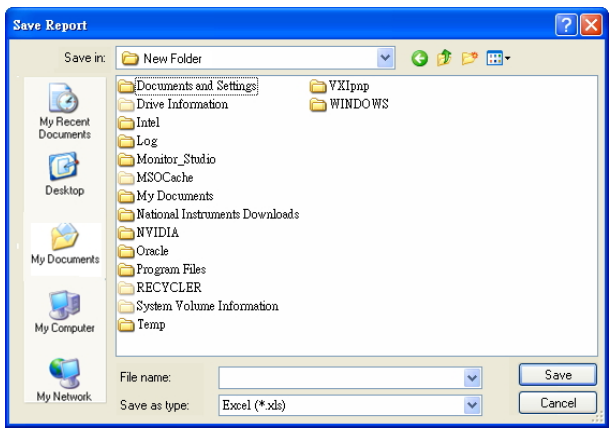
\includegraphics[width=1\linewidth]{Chapters/img/17020_Program/Report/Export_data_analysis.png}
		\centering
		\captionsetup{justification=centering,margin=2cm}
		\caption{หน้าต่างบันทึกข้อมูลจากเมนู Data Analysis}
		\label{fig:Export_data_analysis}
	\end{figure}
\end{center}
































































































































































































































































































